\documentclass[xcolor=dvipsnames]{beamer}

%aspectratio=169
%\usecolortheme[RGB={205,173,0}]{structure} 

% ************************************
% -------------- CONFIGURAÇÔES GERAIS --------
%*************************************
% Definindo novas cores
\usepackage{xcolor}
\definecolor{verde}{rgb}{0.25,0.5,0.35}
\definecolor{jpurple}{rgb}{0.5,0,0.35}
\usepackage[utf8]{inputenc}
\usepackage[portuges]{babel}
%\usepackage{minted}
\usepackage{listings}
\usepackage{graphicx}
\usepackage{tikz}
\usepackage{color}

\lstdefinestyle{Java}
{
  language=Java,
  basicstyle=\ttfamily\small, 
  keywordstyle=\color{jpurple}\bfseries,
  stringstyle=\color{red},
  commentstyle=\color{verde},
  morecomment=[s][\color{blue}]{/**}{*/},
  extendedchars=true, 
  showspaces=false, 
  showstringspaces=false, 
  numbers=left,
  numberstyle=\tiny,
  breaklines=true, 
  backgroundcolor=\color{cyan!10}, 
  breakautoindent=true, 
  captionpos=b,
  xleftmargin=0pt,
  tabsize=4
}

\lstdefinestyle{HTML}
{
	language=HTML,	
	basicstyle=\scriptsize\ttfamily\tiny,
    keywordstyle=\color{jpurple}\bfseries\ttfamily,
    commentstyle=\color{gray}\ttfamily,
	backgroundcolor=\color{cyan!10},
	showspaces=false, 
	extendedchars=true, 	
	showstringspaces=false,
	breakautoindent=true,
	breaklines=true,
	captionpos=b,
    xleftmargin=0pt,
    tabsize=4,
	stringstyle=\color{blue}
	%escapechar=| % Escape to LaTeX between |...|
}


\graphicspath{{img/}}

% ************************************
% -------------- CONFIG BEAMER -------------
%*************************************
\usetheme{Antibes}
\usecolortheme[named=Maroon]{structure}
\setbeamertemplate{blocks}[rounded][shadow=true] 
\setbeamertemplate{navigation symbols}{} 
\useoutertheme{infolines} 


% ************************************
% ------------- INFORMAÇOES PESSOIS -------------
%*************************************
\title{Recomendador de Objetos de Aprendizagem  Baseado em Competências}
\subtitle{Recoacomp}
\author{Rodrigo Freitas Leite}
\institute{UFRGS-NUTED}


% ************************************
% -------------- MACROS -------------
%*************************************
\newcommand{\summarioSectionSubsection}
{
	\begin{frame}
		\frametitle{Sumário}
		\tableofcontents[currentsection,currentsubsection] 
	\end{frame}	
}	
 
\newcommand{\summario}
{
	\begin{frame}
		\frametitle{Sumário}
		\tableofcontents
	\end{frame}	
}	

\newcommand{\summarioSection}
{
	\begin{frame}
		\frametitle{Sumário}
		\tableofcontents[currentsection] 
	\end{frame}	
}	

\newcommand{\actor}[3]
{
	\draw[thick] (#1, #2) -- (#1, #2 + .5);	%neck
	\draw[thick] (#1, #2) -- (#1, #2 - .4);	%tronco  
	\draw[thick] (#1, #2) -- (#1 + .5, #2); %rigth arm
	\draw[thick] (#1, #2) -- (#1 - .5, #2); %left arm
	\draw[thick] (#1, #2 - .4) -- (#1 + .3 ,#2 - 0.9); %leg rigth
	\draw[thick] (#1, #2 - .4) -- (#1 - .3, #2 - 0.9); %leg left 
	\shade[ball color=#3] (#1, {#2 + .6}) circle (.3);

}

\newcommand{\stringBox}[4]
{
	\draw [fill={#4},thick] (#1, #2) rectangle (#1 + 3, #2 + 1);
	\node at (#1 + 1.5, #2 + 0.5) {#3};
}

\newcommand{\stringBoxSmall}[4]
{
	\draw [fill={#4},thick] (#1, #2) rectangle (#1 + 2.5, #2 + 0.5);	
	\node at (#1 + 1.25, #2 + 0.25) {#3};
}

\newcommand{\numberBoxSmall}[4]
{
	\draw [fill={#4},thick] (#1, #2) rectangle (#1 + 1, #2 + 0.5);	
	\node at (#1 + 0.5, #2 + 0.25) {#3};
}

\newcommand{\repositorio}[2]
{
	\draw[thick,fill=SkyBlue] (#1,#2) circle (1.3);
	\shade[ball color=purple] (#1 -0.5, #2 -0.5) circle (0.3);
	\shade[ball color=blue] (#1 +0.5, #2 +0.6) circle (0.3);
	\shade[ball color=pink] (#1 -0.4, #2 +0.8) circle (0.3);
	\shade[ball color=orange] (#1 +0.5, #2 -0.7) circle (0.3);
}

\newcommand{\nota}[4]
{
	\draw[thick, fill=#3] (#1-0.3, #2-0.3) -- (#1, #2+0.3) -- (#1+0.3, #2-0.3) -- cycle;
	\node at (#1,#2-0.1) {#4};	
}

% ************************************
% -------------- SLIDE 1 -------------
%*************************************
\begin{document}

\begin{frame}
	\titlepage
\end{frame}

% ************************************
% -------------- SLIDE 2 -------------
%*************************************

\summario{}

% ************************************
% -------------- SLIDE 3 -------------
%*************************************
\section{Concepção}
	\subsection{Análise de Requisitos}   
	  \begin{frame}{Conceitos}

	     \begin{block}{Objetos de Aprendizagem (OA)}
Objetos de aprendizagem são qualquer entidade, digital ou não digital, que possa ser referenciada durante o aprendizado.
	  	 \end{block}

 	     \begin{block}{Competência}
Competências são um conjunto de elementos compostos pelos Conhecimentos, Habilidades e Atitudes(CHA). Tal conjunto é estruturado e mobilizado em um contexto determinado com o intuito de solucionar um problema e/ou lidar com uma situação nova.
		 \end{block}

		 \begin{block}{Sistema de Recomendação}
Sistema que visa auxiliar o usuário na busca e seleção de um conteúdo, funcionando como um filtro de informação. Assim, o usuário terá como resultado OA mais relevantes, conforme utiliza e alimenta o sistema com novas informações, seja do perfil, seja das pesquisas realizadas.
		\end{block}	
	
	 \end{frame}

% ************************************
% -------------- SLIDE 4 -------------
%*************************************
\begin{frame}{Objetivo}

	\begin{block}{Propósito}
O recomendador deve fornecer Objetos de Aprendizagem que supram a necessidade das competências do usuário, ou seja, o recomendador ajuda o usuário a construir suas competências.
	\end{block}

\end{frame}


% ************************************
% -------------- SLIDE 5 -------------
%*************************************
\subsection{Caso de Uso}
	\begin{frame}{Cenário Básico}

	\begin{tikzpicture}
			% Usuario da direita		
		\numberBoxSmall{8}{6.6}{5}{yellow}	
		\stringBoxSmall{9}{6.6}{Atitude}{yellow}
		
		\numberBoxSmall{8}{7.1}{2}{yellow}	
		\stringBoxSmall{9}{7.1}{Habilidade}{yellow}	
		
		\numberBoxSmall{8}{7.6}{3}{yellow}	
		\stringBoxSmall{9}{7.6}{Conhecimento}{yellow}
				
		\stringBoxSmall{8.55}{8.1}{Reflexão}{yellow}	
		
		\actor{10.5}{5}{yellow}

			% Usuario da esquerda
		\numberBoxSmall{2.5}{6.6}{3}{green}	
		\stringBoxSmall{0}{6.6}{Atitude}{green}
		
		\numberBoxSmall{2.5}{7.1}{2}{green}	
		\stringBoxSmall{0}{7.1}{Habilidade}{green}	
		
		\numberBoxSmall{2.5}{7.6}{7}{green}	
		\stringBoxSmall{0}{7.6}{Conhecimento}{green}	

		\stringBoxSmall{0.5}{8.1}{Reflexão}{green}	
		
		\actor{1.5}{5}{green}

			% Recomendador
		\stringBox{2.5}{2.5}{Recoacomp}{Apricot}

		\repositorio{8.5}{2.5}		
		\stringBoxSmall{9.7}{1.5}{Repositório}{SkyBlue}	

		%\draw[ultra thick, <-] (1,-2) to (4,-3);
	\end{tikzpicture}

	\end{frame}

% ************************************
% -------------- SLIDE 6 -------------
%*************************************	
	\begin{frame}{Análise das Competências dos Usuários}

	\begin{tikzpicture}
		\numberBoxSmall{8}{6.6}{5}{yellow}	
		\stringBoxSmall{9}{6.6}{Atitude}{yellow}
		
		\numberBoxSmall{8}{7.1}{2}{yellow}	
		\stringBoxSmall{9}{7.1}{Habilidade}{yellow}	
		
		\numberBoxSmall{8}{7.6}{3}{yellow}	
		\stringBoxSmall{9}{7.6}{Conhecimento}{yellow}
				
		\stringBoxSmall{8.55}{8.1}{Reflexão}{yellow}	
		
		\actor{10.5}{5}{yellow}

			% Usuario da esquerda
		\numberBoxSmall{2.5}{6.6}{3}{green}	
		\stringBoxSmall{0}{6.6}{Atitude}{green}
		
		\numberBoxSmall{2.5}{7.1}{2}{green}	
		\stringBoxSmall{0}{7.1}{Habilidade}{green}	
		
		\numberBoxSmall{2.5}{7.6}{7}{green}	
		\stringBoxSmall{0}{7.6}{Conhecimento}{green}	

		\stringBoxSmall{0.5}{8.1}{Reflexão}{green}	
		
		\actor{1.5}{5}{green}

			% Recomendador
		\stringBox{2.5}{2.5}{Recoacomp}{Apricot}

		\draw[ultra thick, ->] (5,3.5) to (8,7.5);
		\draw[ultra thick, ->] (4,3.5) to (3,6.6);
	
		\repositorio{8.5}{2.5}		
		\stringBoxSmall{9.7}{1.5}{Repositório}{SkyBlue}	
			
	\end{tikzpicture}

\end{frame}

% ************************************
% -------------- SLIDE 7 -------------
%*************************************	
	\begin{frame}{Busca no Repositório por Objetos de Aprendizagem}

	\begin{tikzpicture}
		\numberBoxSmall{8}{6.6}{5}{yellow}	
		\stringBoxSmall{9}{6.6}{Atitude}{yellow}
		
		\numberBoxSmall{8}{7.1}{2}{yellow}	
		\stringBoxSmall{9}{7.1}{Habilidade}{yellow}	
		
		\numberBoxSmall{8}{7.6}{3}{yellow}	
		\stringBoxSmall{9}{7.6}{Conhecimento}{yellow}
				
		\stringBoxSmall{8.55}{8.1}{Reflexão}{yellow}	
		
		\actor{10.5}{5}{yellow}

			% Usuario da esquerda
		\numberBoxSmall{2.5}{6.6}{3}{green}	
		\stringBoxSmall{0}{6.6}{Atitude}{green}
		
		\numberBoxSmall{2.5}{7.1}{2}{green}	
		\stringBoxSmall{0}{7.1}{Habilidade}{green}	
		
		\numberBoxSmall{2.5}{7.6}{7}{green}	
		\stringBoxSmall{0}{7.6}{Conhecimento}{green}	

		\stringBoxSmall{0.5}{8.1}{Reflexão}{green}	
		
		\actor{1.5}{5}{green}

			% Recomendador
		\stringBox{2.5}{2.5}{Recoacomp}{Apricot}

		\repositorio{8.5}{2.5}		
		\stringBoxSmall{9.7}{1.5}{Repositório}{SkyBlue}	
	
		\draw[ultra thick, ->] (5.5,3) to (7.2,2.7);	
			
	\end{tikzpicture}

\end{frame}

% ************************************
% -------------- SLIDE 8 -------------
%*************************************
\begin{frame}{Recomendação de Objetos de Aprendizagem}

	\begin{tikzpicture}
		\numberBoxSmall{8}{6.6}{5}{yellow}	
		\stringBoxSmall{9}{6.6}{Atitude}{yellow}
		
		\numberBoxSmall{8}{7.1}{2}{yellow}	
		\stringBoxSmall{9}{7.1}{Habilidade}{yellow}	
		
		\numberBoxSmall{8}{7.6}{3}{yellow}	
		\stringBoxSmall{9}{7.6}{Conhecimento}{yellow}
				
		\stringBoxSmall{8.55}{8.1}{Reflexão}{yellow}	
		
		\actor{10.5}{5}{yellow}

			% Usuario da esquerda
		\numberBoxSmall{2.5}{6.6}{3}{green}	
		\stringBoxSmall{0}{6.6}{Atitude}{green}
		
		\numberBoxSmall{2.5}{7.1}{2}{green}	
		\stringBoxSmall{0}{7.1}{Habilidade}{green}	
		
		\numberBoxSmall{2.5}{7.6}{7}{green}	
		\stringBoxSmall{0}{7.6}{Conhecimento}{green}	

		\stringBoxSmall{0.5}{8.1}{Reflexão}{green}	
		
		\actor{1.5}{5}{green}

			% Recomendador
		\stringBox{2.5}{2.5}{Recoacomp}{Apricot}

		\repositorio{8.5}{2.5}		
		\stringBoxSmall{9.7}{1.5}{Repositório}{SkyBlue}	
	
		\draw[ultra thick, ->] (5,3.5) to (7.5,6.5);
		\draw[ultra thick, ->] (4,3.5) to (3.89,6.8);		
		
		\shade[ball color=purple] (7.6, 6.8) circle (0.25);
		\shade[ball color=blue] (7.6, 7.33) circle (0.25);
		
		\shade[ball color=pink] (3.9, 7.85) circle (0.25);
		\shade[ball color=blue] (3.9, 7.3) circle (0.25);
	
	\end{tikzpicture}

\end{frame}

% ************************************
% -------------- SLIDE 9 -------------
%*************************************
\begin{frame}{Avaliação dos Objetos de Aprendizagem pelos Usuários}

	\begin{tikzpicture}
		\numberBoxSmall{8}{6.6}{5}{yellow}	
		\stringBoxSmall{9}{6.6}{Atitude}{yellow}
		
		\numberBoxSmall{8}{7.1}{2}{yellow}	
		\stringBoxSmall{9}{7.1}{Habilidade}{yellow}	
		
		\numberBoxSmall{8}{7.6}{3}{yellow}	
		\stringBoxSmall{9}{7.6}{Conhecimento}{yellow}
				
		\stringBoxSmall{8.55}{8.1}{Reflexão}{yellow}	
		
		\actor{10.5}{5}{yellow}

			% Usuario da esquerda
		\numberBoxSmall{2.5}{6.6}{3}{green}	
		\stringBoxSmall{0}{6.6}{Atitude}{green}
		
		\numberBoxSmall{2.5}{7.1}{2}{green}	
		\stringBoxSmall{0}{7.1}{Habilidade}{green}	
		
		\numberBoxSmall{2.5}{7.6}{7}{green}	
		\stringBoxSmall{0}{7.6}{Conhecimento}{green}	

		\stringBoxSmall{0.5}{8.1}{Reflexão}{green}	
		
		\actor{1.5}{5}{green}

			% Recomendador
		\stringBox{2.5}{2.5}{Recoacomp}{Apricot}

		\repositorio{8.5}{2.5}		
		\stringBoxSmall{9.7}{1.5}{Repositório}{SkyBlue}	
	
		\draw[ultra thick, ->] (1.9,4.5) to (3.85,7);
		\draw[ultra thick, ->] (10,4.7) to (7.8,6.5);		
		
		\shade[ball color=purple] (7.6, 6.8) circle (0.25);
		\shade[ball color=blue] (7.6, 7.33) circle (0.25);
		
		\shade[ball color=pink] (3.9, 7.85) circle (0.25);
		\shade[ball color=blue] (3.9, 7.3) circle (0.25);

		\nota{4.5}{8.1}{green}{2}
		\nota{4.5}{7.4}{green}{3}

		\nota{7}{7.5}{yellow}{2}
		\nota{7}{6.8}{yellow}{4}

	\end{tikzpicture}

\end{frame}

% ************************************
% -------------- SLIDE 10 -------------
%*************************************
\begin{frame}{Filtragem Colaborativa - Grau de Similaridade}

	\begin{tikzpicture}
		\numberBoxSmall{8}{6.6}{5}{yellow}	
		\stringBoxSmall{9}{6.6}{Atitude}{yellow}
		
		\numberBoxSmall{8}{7.1}{2}{yellow}	
		\stringBoxSmall{9}{7.1}{Habilidade}{yellow}	
		
		\numberBoxSmall{8}{7.6}{3}{yellow}	
		\stringBoxSmall{9}{7.6}{Conhecimento}{yellow}
				
		\stringBoxSmall{8.55}{8.1}{Reflexão}{yellow}	
		
		\actor{10.5}{5}{yellow}

			% Usuario da esquerda
		\numberBoxSmall{2.5}{6.6}{3}{green}	
		\stringBoxSmall{0}{6.6}{Atitude}{green}
		
		\numberBoxSmall{2.5}{7.1}{2}{green}	
		\stringBoxSmall{0}{7.1}{Habilidade}{green}	
		
		\numberBoxSmall{2.5}{7.6}{7}{green}	
		\stringBoxSmall{0}{7.6}{Conhecimento}{green}	

		\stringBoxSmall{0.5}{8.1}{Reflexão}{green}	
		
		\actor{1.5}{5}{green}

			% Recomendador
		\stringBox{2.5}{2.5}{Recoacomp}{Apricot}

		\repositorio{8.5}{2.5}		
		\stringBoxSmall{9.7}{1.5}{Repositório}{SkyBlue}	
	
		\shade[ball color=purple] (7.6, 6.8) circle (0.25);
		\shade[ball color=blue] (7.6, 7.33) circle (0.25);
		
		\shade[ball color=pink] (3.9, 7.85) circle (0.25);
		\shade[ball color=blue] (3.9, 7.3) circle (0.25);

		\nota{4.5}{8.1}{green}{2}
		\nota{4.5}{7.4}{green}{3}

		\nota{7}{7.5}{yellow}{2}
		\nota{7}{6.8}{yellow}{4}

		\draw[ultra thick, <->] (4.7,7.5) to (6.8,7.5);
		

	\end{tikzpicture}

\end{frame}

% ************************************
% -------------- SLIDE 11 -------------
%*************************************
\begin{frame}{Filtragem Colaborativa - Recomendação}

	\begin{tikzpicture}
		\numberBoxSmall{8}{6.6}{5}{yellow}	
		\stringBoxSmall{9}{6.6}{Atitude}{yellow}
		
		\numberBoxSmall{8}{7.1}{2}{yellow}	
		\stringBoxSmall{9}{7.1}{Habilidade}{yellow}	
		
		\numberBoxSmall{8}{7.6}{3}{yellow}	
		\stringBoxSmall{9}{7.6}{Conhecimento}{yellow}
				
		\stringBoxSmall{8.55}{8.1}{Reflexão}{yellow}	
		
		\actor{10.5}{5}{yellow}

			% Usuario da esquerda
		\numberBoxSmall{2.5}{6.6}{3}{green}	
		\stringBoxSmall{0}{6.6}{Atitude}{green}
		
		\numberBoxSmall{2.5}{7.1}{2}{green}	
		\stringBoxSmall{0}{7.1}{Habilidade}{green}	
		
		\numberBoxSmall{2.5}{7.6}{7}{green}	
		\stringBoxSmall{0}{7.6}{Conhecimento}{green}	

		\stringBoxSmall{0.5}{8.1}{Reflexão}{green}	
		
		\actor{1.5}{5}{green}

			% Recomendador
		\stringBox{2.5}{2.5}{Recoacomp}{Apricot}

		\repositorio{8.5}{2.5}		
		\stringBoxSmall{9.7}{1.5}{Repositório}{SkyBlue}	
	
		\shade[ball color=purple] (7.6, 6.8) circle (0.25);
		\shade[ball color=blue] (7.6, 7.33) circle (0.25);
		
		\shade[ball color=pink] (3.9, 7.85) circle (0.25);
		\shade[ball color=blue] (3.9, 7.3) circle (0.25);

		\nota{4.5}{8.1}{green}{1}
		\nota{4.5}{7.4}{green}{3}

		\nota{7}{7.5}{yellow}{3}
		\nota{7}{6.8}{yellow}{4}

		\draw[ultra thick, ->] (4.7,8) to (6.7,8);
		\draw[ultra thick, <-] (4.8,6.78) to (6.82,6.78);
		
		\shade[ball color=purple] (3.9, 6.78) circle (0.25);
		\shade[ball color=pink] (7.6, 7.85) circle (0.25);

		\nota{7}{8.15}{yellow}{}
		\nota{4.5}{6.8}{green}{}

	\end{tikzpicture}

\end{frame}


% ************************************
% -------------- SLIDE 12 -------------
%*************************************
\begin{frame}{Filtragem Colaborativa - FeedBack dos Usuários}

	\begin{tikzpicture}
		\numberBoxSmall{8}{6.6}{5}{yellow}	
		\stringBoxSmall{9}{6.6}{Atitude}{yellow}
		
		\numberBoxSmall{8}{7.1}{2}{yellow}	
		\stringBoxSmall{9}{7.1}{Habilidade}{yellow}	
		
		\numberBoxSmall{8}{7.6}{3}{yellow}	
		\stringBoxSmall{9}{7.6}{Conhecimento}{yellow}
				
		\stringBoxSmall{8.55}{8.1}{Reflexão}{yellow}	
		
		\actor{10.5}{5}{yellow}

			% Usuario da esquerda
		\numberBoxSmall{2.5}{6.6}{3}{green}	
		\stringBoxSmall{0}{6.6}{Atitude}{green}
		
		\numberBoxSmall{2.5}{7.1}{2}{green}	
		\stringBoxSmall{0}{7.1}{Habilidade}{green}	
		
		\numberBoxSmall{2.5}{7.6}{7}{green}	
		\stringBoxSmall{0}{7.6}{Conhecimento}{green}	

		\stringBoxSmall{0.5}{8.1}{Reflexão}{green}	
		
		\actor{1.5}{5}{green}

			% Recomendador
		\stringBox{2.5}{2.5}{Recoacomp}{Apricot}

		\repositorio{8.5}{2.5}		
		\stringBoxSmall{9.7}{1.5}{Repositório}{SkyBlue}	
	
		\shade[ball color=purple] (7.6, 6.8) circle (0.25);
		\shade[ball color=blue] (7.6, 7.33) circle (0.25);
		
		\shade[ball color=pink] (3.9, 7.85) circle (0.25);
		\shade[ball color=blue] (3.9, 7.3) circle (0.25);

		\nota{4.5}{8.1}{green}{1}
		\nota{4.5}{7.4}{green}{3}

		\nota{7}{7.5}{yellow}{3}
		\nota{7}{6.8}{yellow}{4}

		\shade[ball color=purple] (3.9, 6.78) circle (0.25);
		\shade[ball color=pink] (7.6, 7.85) circle (0.25);

		\nota{7}{8.15}{yellow}{5}
		\nota{4.5}{6.8}{green}{4}

		\draw[ultra thick, ->] (1.9,4.4) to (3.85,6.5);
		\draw[ultra thick, ->] (10,4.7) to (7.8,6.5);		

	\end{tikzpicture}

\end{frame}


% ************************************
% -------------- SLIDE 13 -------------
%*************************************
\section{Projeto e Desenvolvimento}
   \subsection{Pradrão Arquitetural}
	\begin{frame}{Model View Controller - MVC}
		\begin{block}{JavaServer Faces - JSF}	
É um framework MVC baseado em Java para a construção de interfaces de usuário baseadas em componentes para aplicações web. Possui um modelo de programação dirigido a eventos, abstraindo os detalhes da manipulação dos eventos e organização dos componentes, permitindo que o programador se concentre na lógica da aplicação.	
		\end{block}
	\end{frame}

% ************************************
% -------------- SLIDE 14 -------------
%*************************************
	\begin{frame}{MVC Pull - Action Based}
		\begin{figure}[!htb]
			\centering
			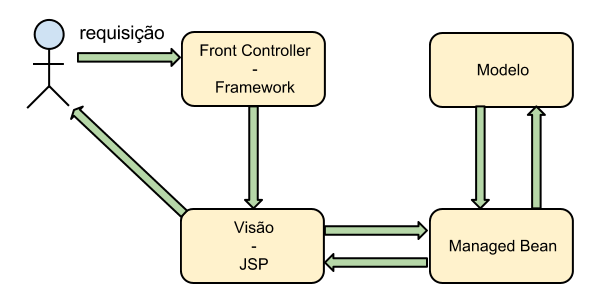
\includegraphics[keepaspectratio=true,height=5cm]{mvc-pull.png}
			\caption{Modelo MVC Pull}
			\label{rec-ER}
		\end{figure}				

	\end{frame}	

% ************************************
% -------------- SLIDE 15 -------------
%*************************************
\subsection{MVC}
	\begin{frame}[fragile]{View}
		\begin{block}{Facelets}
Facelets é uma linguagem de declaração página, que é usado para construir JavaServer Faces exibições usando modelos de estilo HTML e para a construção de árvores de componentes.
		\end{block}
	\end{frame}	

% ************************************
% -------------- SLIDE 16 -------------
%*************************************
\begin{frame}[fragile]{Facelets - Página}
		
	\begin{lstlisting}[style=HTML]
<!DOCTYPE html PUBLIC "-//W3C//DTD XHTML 1.0 Transitional//EN"
 "http://www.w3.org/TR/xhtml1/DTD/xhtml1-transitional.dtd"> 
<html xmlns="http://www.w3.org/1999/xhtml"
      xmlns:h="http://java.sun.com/jsf/html"
      xmlns:f="http://java.sun.com/jsf/core"
      xmlns:ui="http://java.sun.com/jsf/facelets"> 

<h:head>
	<title>Exemple</title>
</h:head>
 
<h:body> 
	<h:form>
		<h:panelGrid columns="2">
		<h:outputText value="Nome: " />
			<h:inputText value="#{user.name}" />
			<h:outputText value="Email: " />
			<h:inputText value="#{user.email}" />		
		</h:panelGrid>
		<h:commandButton value="action" action="#{user.action()}" />
	</h:form>
</h:body> 
</html>
	\end{lstlisting}		

\end{frame}

% ************************************
% -------------- SLIDE 17 -------------
%*************************************
\begin{frame}{Página}
	\begin{figure}[!htb]
		\centering
		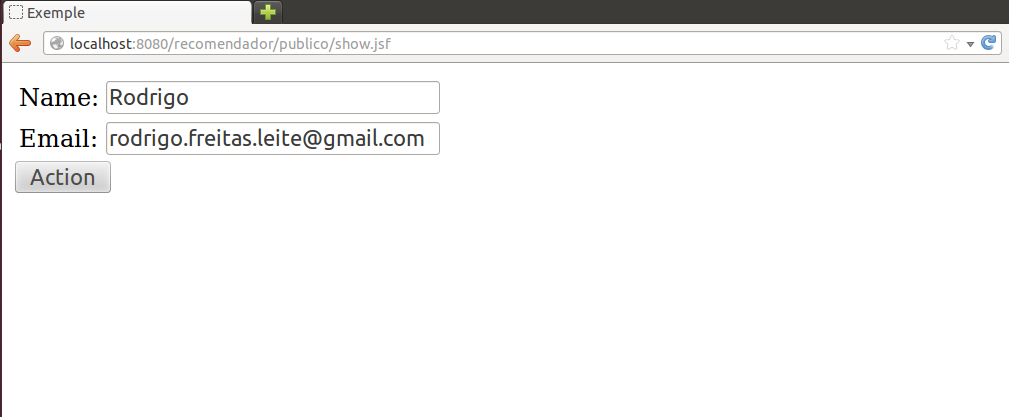
\includegraphics[keepaspectratio=true,height=5cm]{facelets-1rec.png}
		\caption{Página Gerada}
		\label{rec-ER}
\end{figure}

		\end{frame}

% ************************************
% -------------- SLIDE 18 -------------
%*************************************
\begin{frame}[fragile]{Criando Componente}
	\begin{lstlisting}[style=HTML]
<!DOCTYPE html PUBLIC "-//W3C//DTD XHTML 1.0 Transitional//EN"
"http://www.w3.org/TR/xhtml1/DTD/xhtml1-transitional.dtd">
<html xmlns="http://www.w3.org/1999/xhtml"
      xmlns:h="http://java.sun.com/jsf/html"
      xmlns:composite="http://java.sun.com/jsf/composite"
      xmlns:f="http://java.sun.com/jsf/core"
      xmlns:ui="http://java.sun.com/jsf/facelets">
<body>

<composite:interface>

		<composite:attribute name="typeAction" />

</composite:interface>
<composite:implementation>

	<h:panelGrid columns="2" >
			<h:outputText value="Name: " />
			<h:inputText value="#{user.name}" />
			<h:outputText value="Email: " />
			<h:inputText value="#{user.email}" />		
	</h:panelGrid>
	<h:commandButton value="#{cc.attrs.typeAction}" action="#{user.action()}" />

</composite:implementation>

</body>
</html>	
	\end{lstlisting}
\end{frame}




% ************************************
% -------------- SLIDE 19 -------------
%*************************************
\begin{frame}[fragile]{Utilizando Componente}
	\begin{lstlisting}[style=HTML]
<!DOCTYPE html PUBLIC "-//W3C//DTD XHTML 1.0 Transitional//EN"
 "http://www.w3.org/TR/xhtml1/DTD/xhtml1-transitional.dtd"> 
<html xmlns="http://www.w3.org/1999/xhtml"
      xmlns:h="http://java.sun.com/jsf/html"
      xmlns:f="http://java.sun.com/jsf/core"
      xmlns:ui="http://java.sun.com/jsf/facelets"
      xmlns:util="http://java.sun.com/jsf/composite/components/util"> 
<h:head>
	<title>Exemple</title>
</h:head> 
<h:body> 
	<h:form >
		<util:componente  typeAction="Save" />
		<util:componente typeAction="Update" />
	</h:form>
</h:body> 
</html>
	\end{lstlisting}
\end{frame}

% ************************************
% -------------- SLIDE 20 -------------
%*************************************
\begin{frame}{Página com Componente}
	\begin{figure}[!htb]
		\centering
		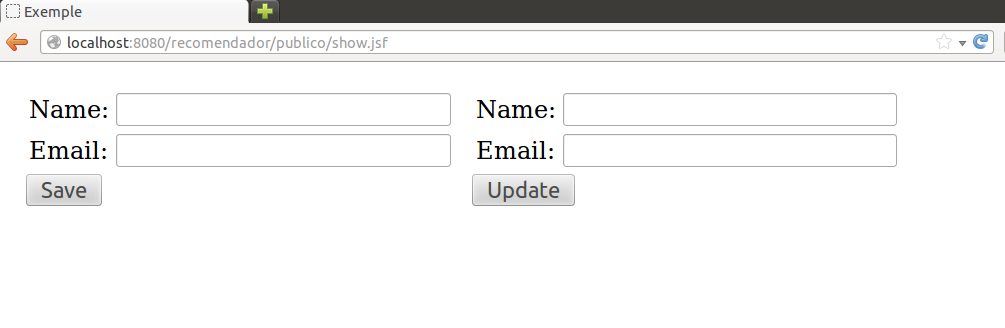
\includegraphics[keepaspectratio=true,height=3.5cm]{facelets-2rec.png}
		\caption{Página com Componente}
		\label{rec-ER}
\end{figure}

		\end{frame}




% ************************************
% -------------- SLIDE 21 -------------
%*************************************
\subsection{Modelagem de Entidades}
		\begin{frame}{Diagrama Entidade-Relacionamento}

\begin{figure}[!htb]
	\centering
	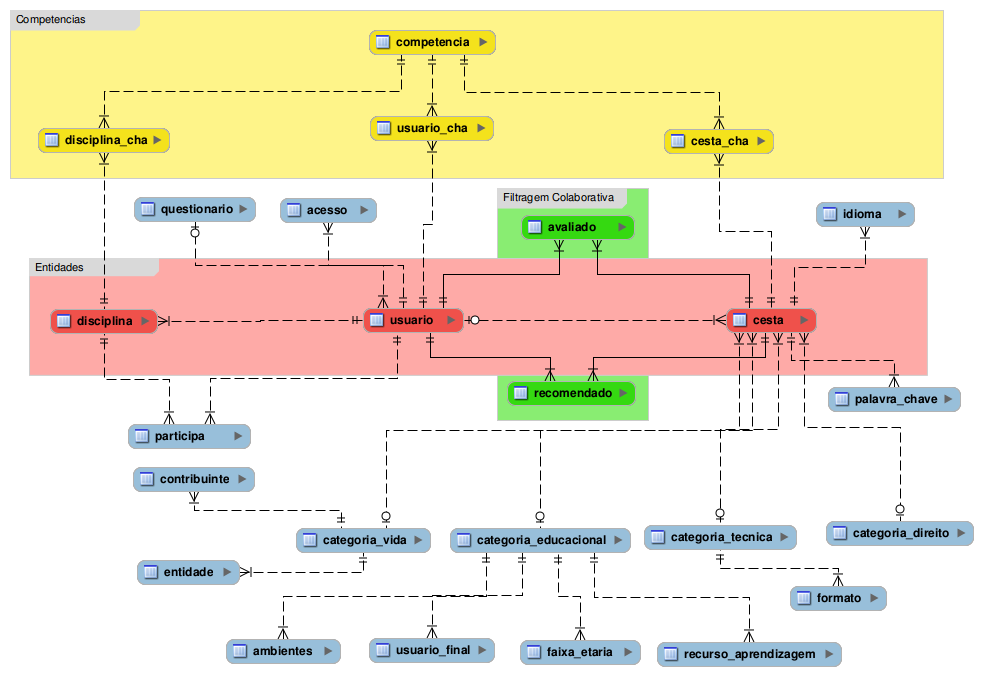
\includegraphics[keepaspectratio=true,height=6.7cm]{recomendador-ER.png}
	\caption{Diagrama de Entidade Relacionamento}
	\label{rec-ER}
\end{figure}

		\end{frame}

% ************************************
% -------------- SLIDE 22 -------------
%*************************************
\begin{frame}{Mapeamento Objeto Relacional}
	

	\begin{block}{Java Persistence API}
É uma especificação que descreve o gerenciamento de dados relacionais em aplicações. Tal gerenciamento é realizado de maneira automatizada e transparente para tabelas em um banco de dados relacional, usando metadados que descrevem o mapeamento entre objetos e o banco de dados.	
	\end{block}		

\end{frame}	

% ************************************
% -------------- SLIDE 23 -------------
%*************************************
\begin{frame}[fragile]{Mapeamento Objeto Relacional}
	\begin{columns}[c]
		\column{.6\textwidth}	
			\begin{lstlisting}[style=Java]
@Entity
public class usuario {
	@Id
	@Column
	private int id;

	@Column
	private String nome;

	@Column
	private String senha;
		
	@Column
	private String email;		
	
	@OneToMany
	private List<UsuarioCha> cha;
}
			\end{lstlisting}							
		\column{.3\textwidth}
			\begin{figure}[!htb]
				\centering
				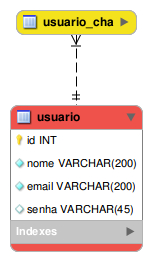
\includegraphics[keepaspectratio=true,height=5cm]{usuario-ER.png}
				\caption{Tabela Usuario}
				\label{usuario-ER}
			\end{figure}	
	\end{columns}
\end{frame}

% ************************************
% -------------- SLIDE 24 -------------
%*************************************



% ************************************
% -------------- SLIDE Final -------------
%*************************************
\section{Conclusão}
	\begin{frame}{Perguntas?}
		\titlepage
		\begin{center}					
		 \href{mailto:rodrigo.freitas.leite@gmail.com}{rodrigo.freitas.leite@gmail.com}	
		\end{center}
			
	\end{frame}

\end{document}


